\documentclass{article}%
\usepackage[T1]{fontenc}%
\usepackage[utf8]{inputenc}%
\usepackage{lmodern}%
\usepackage{textcomp}%
\usepackage{lastpage}%
\usepackage{authblk}%
\usepackage{graphicx}%
%
\title{Reactive Oxygen Species{-}Triggered Trophoblast Apoptosis Is Initiated by Endoplasmic Reticulum Stress via Activation of Caspase{-}12, CHOP and the JNK Pathway in Toxoplasma gondii Infection in Mice}%
\author{Brian Bennett}%
\affil{Department of Animal and Poultry Sciences, Virginia Tech, Blacksburg, Virginia, United States of America}%
\date{01{-}01{-}2008}%
%
\begin{document}%
\normalsize%
\maketitle%
\section{Abstract}%
\label{sec:Abstract}%
A model of the MOU001 gene therapy used for the treatment of myeloma and other chronic blood disorders appears to simulate the protein synthesis of an RNA messenger in healthy cells, a step in the ongoing development of an RNA switch that delivers gene{-}building instructions to an affected cell from inattention. This research appears in the Dec. 26 online issue of the Journal of Immunology.\newline%
The work on MOU001 is the first to demonstrate that an RNA pathway is indirectly involved in the development of pluripotent stem cells (Pluripotent Stem cells), even when tissues are the same size, according to Traphagen S. Littali, assistant professor of cell biology, DSEE, John A. Henderson Professor of Immunology and assistant dean for research and graduate studies at UC San Diego. He is also a senior investigator in the UCSD{-}led ONTAP Center for Genomic Genetics, a multidisciplinary network of collaborators worldwide that specializes in translational research.\newline%
Pluripotent stem cells are extremely versatile, capable of carrying many different functions, including making and repairing DNA and encoding proteins. Their existence is known primarily from embryonic stem cells that lack the inhibitory function needed to turn embryonic stem cells into a mature embryo.\newline%
The dominant type of embryonic stem cell in the lab is induced pluripotent stem cells (iPSCs), cells derived from adult skin cells. According to Littali, the iPSCs are unique because they are more mature than embryonic stem cells and retain the ability to make and repair DNA and proteins.\newline%
Littali and his colleagues took advantage of the differences in how iPSCs adapt to external stimuli  tissues, brain or other organs  and how they react to different kinds of genes.\newline%
Littali first decoded a gene called MOU001, found in normal adult stem cells of certain tissues and healthy human blood. Now the team analyzed MOU001.\newline%
In normal MOU001, the chemical reactance of DNA entered the cell's nucleus by "selecting" a defective RNA (genetic code) on a methyl group. Littali and his colleagues then identified a signaling protein called TREM (trans RNA protease) that is involved in stopping this enzyme from binding to MOU001.\newline%
In cells that lacked either MOU001 or TREM, however, MOU001 interacted with TREM, and that was exactly the same as in healthy cells without MOU001.\newline%
"Rather than trying to override the idea that a gene can't be turned off or on, this suggests it is very strongly reactive to TREM," Littali said.\newline%
Littali and his colleagues then found evidence that the tRNA turned on some of the proteins in the expression of MOU001, suggesting that TREM interacted with the tRNA in MOU001 to cut off MOU001, disrupting MOU001's normal function.\newline%
"This tells us that using these short molecules to disable MOU001 was likely to be a more efficient or effective therapeutic," Littali said.\newline%
This work is the first evidence that existing gene transcriptional switches may be essentially reversed by drug treatments, rather than just removed or altered. Littali said he is interested in investigating how tRNA pairs tend to repeat themselves.\newline%
Littali said the next step is to develop ways to reverse the transcriptional stimulus in a way that doesn't cause MOU001 to shut down, and then to enable TREM to transfer directly to MOU001 and replace it as a master transcriber.\newline%
\#\#\#

%
\subsection{Image Analysis}%
\label{subsec:ImageAnalysis}%


\begin{figure}[h!]%
\centering%
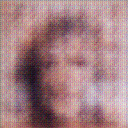
\includegraphics[width=150px]{500_fake_images/samples_5_451.png}%
\caption{A Close Up Of A Small Black And White Cat}%
\end{figure}

%
\end{document}